In this chapter we present the PREcision Timed (PRET) Machine. 
Lorem ipsum dolor sit amet, consectetur adipiscing elit. Nam eu est neque. Suspendisse mollis gravida mi in blandit. Vivamus porta libero at massa sagittis pellentesque. Lorem ipsum dolor sit amet, consectetur adipiscing elit. Sed nibh magna, facilisis ac dapibus vitae, tincidunt nec magna. Morbi ac neque in est porta placerat. Duis viverra blandit ante, ut scelerisque arcu sodales vel. Aenean sapien erat, tincidunt malesuada accumsan a, eleifend feugiat leo. Maecenas auctor nulla non purus fringilla nec hendrerit massa facilisis. Donec vel diam nibh. Maecenas sed massa non mauris faucibus condimentum et et metus. Fusce placerat, dolor et adipiscing suscipit, orci lectus fringilla mauris, a tincidunt dolor mauris id ligula. Vestibulum luctus, dolor in bibendum accumsan, leo turpis suscipit enim, et hendrerit odio metus eget dolor. Morbi in lectus massa.

Lorem ipsum dolor sit amet, consectetur adipiscing elit. Nam eu est neque. Suspendisse mollis gravida mi in blandit. Vivamus porta libero at massa sagittis pellentesque. Lorem ipsum dolor sit amet, consectetur adipiscing elit. Sed nibh magna, facilisis ac dapibus vitae, tincidunt nec magna. Morbi ac neque in est porta placerat. Duis viverra blandit ante, ut scelerisque arcu sodales vel. Aenean sapien erat, tincidunt malesuada accumsan a, eleifend feugiat leo. Maecenas auctor nulla non purus fringilla nec hendrerit massa facilisis. Donec vel diam nibh. Maecenas sed massa non mauris faucibus condimentum et et metus. Fusce placerat, dolor et adipiscing suscipit, orci lectus fringilla mauris, a tincidunt dolor mauris id ligula. Vestibulum luctus, dolor in bibendum accumsan, leo turpis suscipit enim, et hendrerit odio metus eget dolor. Morbi in lectus massa.
\section{Architecture Design\todo{Use repeatability? predictability? analyzability?}}
%Talk about how this allows us to maintain non-interference, and that it allows separate timing analysis
%The thread interleaving pipeline design allows for predictable timing analysis for all threads within the pipeline. 
It is important to understand why and how current architectures fall short of timing predictability and repeatability.
Thus, before we preset the PRET architecture, we briefly discuss common architectural designs and their effects on execution time, and point out some key issues and trade-offs when designing architectures for predictable and repeatable timing.
The introduction of pipelining vastly improved architecture average-case performance.
It allowed faster clock speeds for processors, and improved the instruction throughput compared to single cycle architectures.
Pipelining the datapath allowed subsequent instructions to begin execution while prior instructions were still being completed. 
Ideally each processor cycle one instruction completes and leaves the pipeline as another enters and begins execution. 
In reality, different pipeline hazards occur which reduce the throughput and create stalls in the pipeline.
The handling of these hazards an important factor to the timing predictability and repeatability of the architecture design.     
To illustrate this point, we discuss basic hardware additions proposed to reduce performance penalty from hazards, and their effects on execution time and predictability. 
  
\begin{figure}
\begin{center}
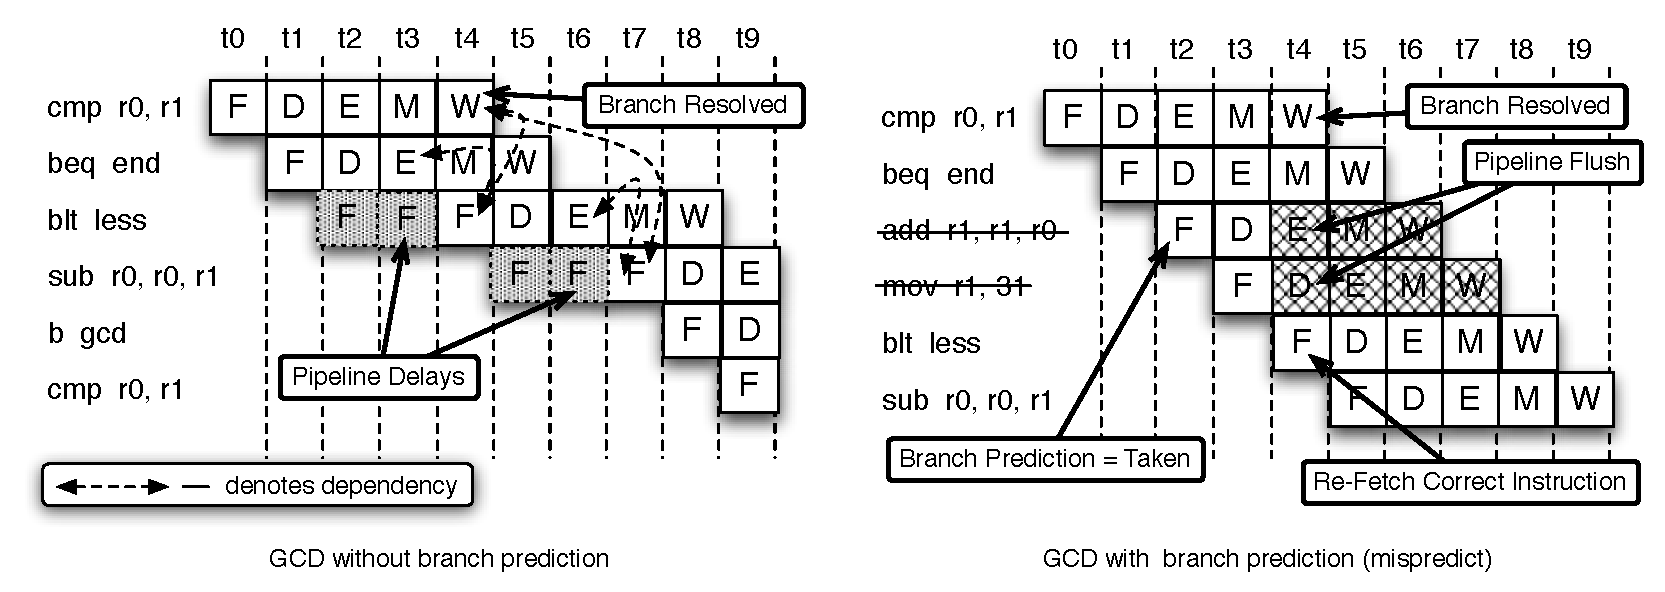
\includegraphics[scale=.58]{figs/branch_execution_non_interleaved_pipeline}
\end{center}
\vspace{-10pt}
\caption{Handling of conditional branches in single threaded pipelines}
\label{fig:branch_execution_non_interleaved_pipeline}
\end{figure}
  
  
\begin{wrapfigure}{r}{0.5\textwidth}
  \vspace{-20pt}
  \begin{center}
    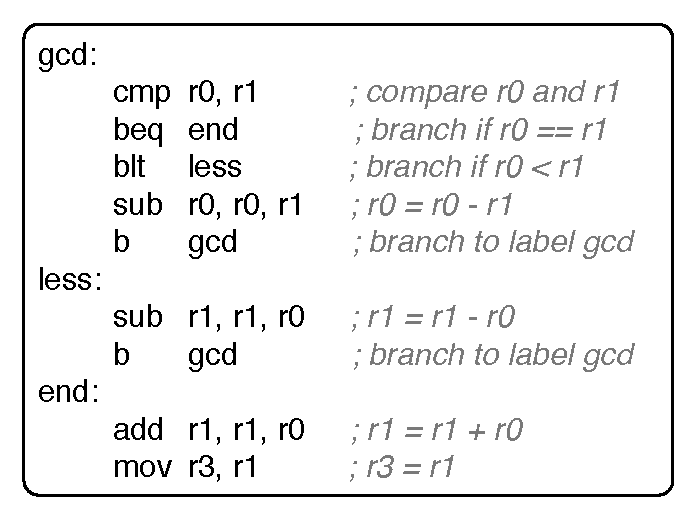
\includegraphics[scale=.65]{figs/sample_gcd_code}
  \end{center}
  \vspace{-20pt}
  \caption{Sample code for GCD with conditional branches}
  \label{fig:sample_gcd_code}
\end{wrapfigure}
We began by looking at how control-flow changes are handled in pipelines.
Branches cause control-flow hazards in the pipeline; the instruction after the branch, which should be fetched the next cycle, is unknown until after the branch instruction is completed.
Conditional branches adds more complexity\todo{?}, as whether or not the branch is taken depends on an additional condition bit. 
The code segment in figure~\ref{fig:sample_gcd_code} shows assembly instructions from the ARM instruction set architecture (ISA) that implement the Greatest Common Divisor (GCD) algorithm using conditional branch instructions \emph{beq} (branch equal) and \emph{blt} (branch less than).  
Conditional branch instructions in ARM branch based on conditional flags that are set with special compare instructions\todo{citation}.
The \emph{cmp} instruction is one such compare instruction that subtracts two registers and updates the conditional flags according to the results.
The GCD implementation shown in the code uses this mechanism to determine whether to continue or end the algorithm.
Figure~\ref{fig:branch_execution_non_interleaved_pipeline} show two ways branches are commonly handled in a single-threaded pipeline. 
In the figure, time progresses horizontally towards the right, each time step, or column, represents a processor cycle.
Each row represents an instruction that is fetched and executed within the pipeline.
Each block represents the instruction entering the different stages of the pipeline -- fetch (F), decode (D), execute (E), memory (M) and writeback (W).   

A simple but effective way of handling control-flow hazards is by simply stalling the pipeline until the branch instruction completes.
This is shown on the left of figure~\ref{fig:branch_execution_non_interleaved_pipeline}. 
Two pipeline delays (or bubbles) are inserted after each branch instruction to wait until address calculation is completed.
The dependencies between instructions are also drawn out to make clear why the pipeline bubbles are necessary.
In order for the \emph{blt} instruction to be fetched, its address must be calculated during the execution stage of the \emph{beq} instruction.
At the same time, because \emph{beq} is a conditional branch, whether or not the branch is taken depends on the \emph{cmp} instruction.
The architecture used contain forwarding circuitry, so the addresses calculated by the branch instructions and the results of the \emph{cmp} instruction can be used before the instructions are committed.
The performance penalty incurred is the pipeline delays inserted to wait for the branch address calculation to complete.
Conditional branches will also incur extra delays for deeper pipelines if the branch condition cannot be resolved in time. 
Some architectures enforce the compiler to insert one or more non-dependent instructions after a branch that is always executed before the change in control-flow of the program. 
These are called branch delay slots and can mitigate the branch penalty, but become less effective as pipelines grow deeper by design. 

In attempt to remove the need of inserting pipeline bubbles, branch predictors were invented to predict the results of a branch before it is resolved\todo{citation}.
%Branch predictors have been heavily researched.
Many clever branch predictors have been proposed, and they can accurately predict branches up to 93.5\%\todo{citation}.
%With branch predictor, the pipeline fetches the next instruction based upon the results of the branch prediction, and continues to execute speculatively.
Branch predictors predict the condition and target addresses of branches, so pipelines can speculatively continue execution based upon the prediction.  
If the prediction was correct, no penalty occurs for the branch, and execution simply continues. 
However, when a mispredict occurs, then the speculatively executed instructions need to be flushed and the correct instructions need to be refetched into the pipeline for execution.
The right of figure~\ref{fig:branch_execution_non_interleaved_pipeline} shows the execution of GCD in the case of a branch misprediction.
After the \emph{beq} instruction, the branch is predicted to be taken, and the \emph{add} and \emph{mov} instructions from the label \emph{end} is directly fetched into execution. 
When the \emph{cmp} instruction is completed, a misprediction is detected, so the \emph{add} and \emph{mov} instruction are flushed out of the pipeline while the correct instruction \emph{blt} is immediately re-fetched and execution continues.
The misprediction penalty is typically the number of stages between fetch and execute, as those cycles are wasted executing instructions from an incorrect execution path.
This penalty only occurs on a mispredict, thus branch prediction typically yields better average performance and is preferred for modern architectures.
%However, for more complex architectures with caches or other hardware states, the effects of incorrectly fetched instructions on the state of the processor less well-known and studied. 
Nonetheless, it is important to understand the effects of branch prediction on execution time. 

Typical branch predictors predict branches based upon the history of previous branches encountered.  
As each branch instruction is resolved, the internal state of the predictor, which stores the branch histories, is updated and used to predict the next branch.
This implicitly creates a dependency between branch instructions and their execution history, as the prediction is affected by its history.
In other words, the execution time of a branch instruction will depend on the branch results of previous branch instructions.
During static execution timing analysis, the state of the branch predictor is unknown because is it often infeasible to keep track of execution history so far back.   
There has been work on explicitly modeling branch predictors for execution time analysis\todo{citation}, but the results are \todo{the results of branch predictor modeling for execution time analysis}.
The analysis needs to conservatively account for the potential branch mispredict penalty for each branch, which leads to overestimated execution times.
To make matters worse, as architectures grow in complexity, more internal states exist in architectures that could be affected by the speculative execution. 
For example, cache lines could be evicted when speculatively executing instructions from a mispredicted path, changing the state of the cache.  
%When instructions from the correct execution path are re-fetched at branch resolution, a cache miss could be resulted from the change in cache because of the branch misprediction.    
This makes a tight static execution time analysis extremely difficult, if not impossible; explicitly modeling all hardware states and their effects together often lead to an infeasible explosion in state space. 
On the other hand, although the simple method of inserting pipeline bubbles for branches could lead to more branch penalties, the static timing analysis is precise and straight forward, as no prediction and speculative execution occur. 
In the case of the ARM ISA, the analysis simply accounts for the branch penalty after every branch. 
Additional penalties from a conditional branch can be accounted for by simply checking for instructions that modify the conditional flag above the conditional branch.
We explicitly showed this simple method of handling branches to point out an important trade-off between speculative execution for better average performance and consistent stalling for better predictability.
Average-case performance can be improved by speculation at the cost of predictability and potentially prolonging the worst-case performance.  
The challenge remains to maintain predictability while improving worst-case performance, and how pipeline hazards are handled play an integral part of tackling this challenge.           

\begin{wrapfigure}{r}{0.5\textwidth}
  \vspace{-20pt}
  \begin{center}
    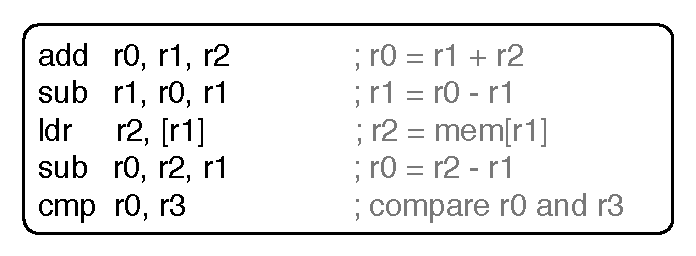
\includegraphics[scale=.65]{figs/sample_data_dependent_code}
  \end{center}
  \vspace{-20pt}
  \caption{Sample code with data dependencies}
  \label{fig:sample_data_dependent_code}
\end{wrapfigure}
Data hazards occur when instructions depend on the results of previous instructions that have yet to commit.
The code segment shown in figure~\ref{fig:sample_data_dependent_code} contains instructions that each depend on the result of its previous instruction.
The top of figure~\ref{fig:data_depend_execution_non_interleaved} shows an execution of the code segment on a naive pipeline without handling of data hazards. 
Data hazards in this case are handled by inserting pipeline delays to ensure the completion of all dependent instructions.
Similar to inserting pipeline delays of control-flow hazards, this method allows for predictable static execution time analysis, but at a slight cost of performance. 
%Figure~\ref{fig:data_depend_execution_non_interleaved} shows the execution of the code segment on pipelines with and without forwarding.
Pipeline forwarding is the most common way of handling data hazards that occur from pipelining.  
A pipeline forwarding circuitry consists of backwards paths for data from different pipeline stages to the inputs of arithmetic units, and multiplexers to select amongst them. 
It provides a way to directly access computation results from the previous instruction before it commits. 
The pipeline controller dynamically detects whether a data-dependency exists, and changes the selection bits to the multiplexers accordingly so the correct operands are selected.
The bottom of figure~\ref{fig:data_depend_execution_non_interleaved} shows the execution with forwarding in the pipeline.
\begin{figure}
\vspace{-20pt}
\begin{center}
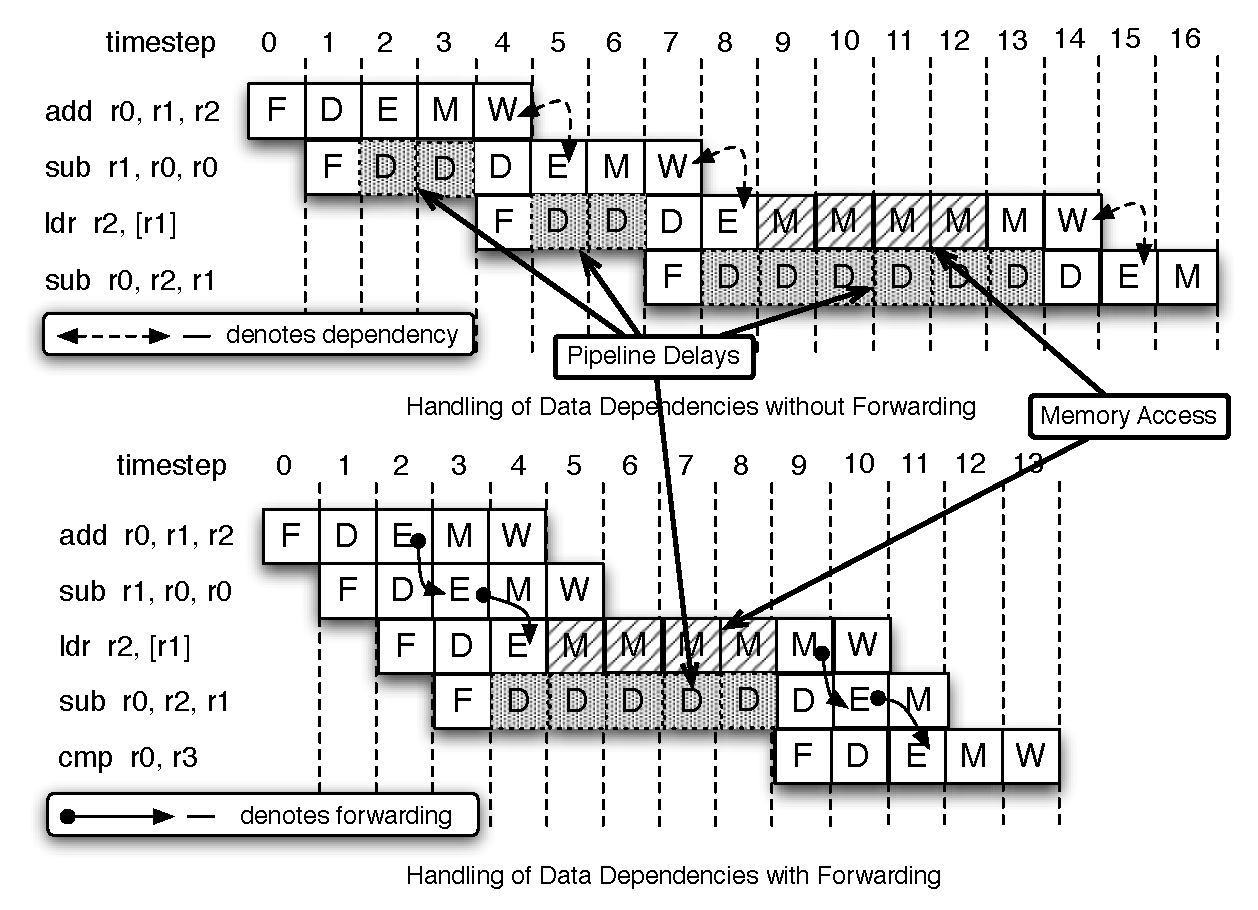
\includegraphics[scale=.6]{figs/data_depend_execution_non_interleaved}
\end{center}
\vspace{-10pt}
\caption{Handling of data dependencies in single threaded pipelines}
\label{fig:data_depend_execution_non_interleaved}
\end{figure}
No pipeline bubbles are needed for the first \emph{sub} instruction and \emph{ld} instruction, as the results they depend on can be computed in one cycle by the ALU, and forwarded through the forwarding paths.
\todo{Needs some reworking here}
Notice that although there is dynamic execution in the pipeline forwarding circuitry, it is actually possible to statically predict the execution time accurately.
The logic in the pipeline controller that enables and selects the correct forwarding bits only needs to check a small set of previous instructions to detect data-dependencies. 
Thus, static execution time analysis can detect forwarding by simply checking a short window of previous instructions to account for stalls accordingly. \todo{find papers to back this up}
The internal state of the branch predictor on the other hand is dependent on branch histories which may have happened arbitrarily long ago in the execution sequence,

\todo{Talk about caches here}
Stalls are still inserted for the the second \emph{sub} instruction, as it is waiting upon the results of a memory operation. 
The memory access latency in the figure is arbitrarily chosen to be 5 cycles for illustrative purposes, but obtaining the actual access latencies of memory operations is a complicated subject which is addressed in section~\ref{subsection:memory_system}.
We can thus see that forwarding can address the data-dependencies caused by pipelining -- the read-after-write of register computations. 
However, they cannot address the data-dependencies caused by other long latency operations such as memory operations, so pipeline stalls are still needed. 
 
Multithreaded architectures were introduced to improve instruction throughput over instruction latency.
The architecture optimizes thread-level parallelism over instruction-level parallelism to improve performance.
Multiple hardware threads are introduced into the pipeline to fully utilize thread-level parallelism. 
When one hardware thread is stalled, another hardware thread can be fetched into the pipeline for execution to avoid stalling the whole pipeline. 
To lower the context switching overhead, the pipeline contains physically separate copies of hardware thread states, such as registers files and program counters etc, for each hardware thread.
\begin{figure}
\begin{center}
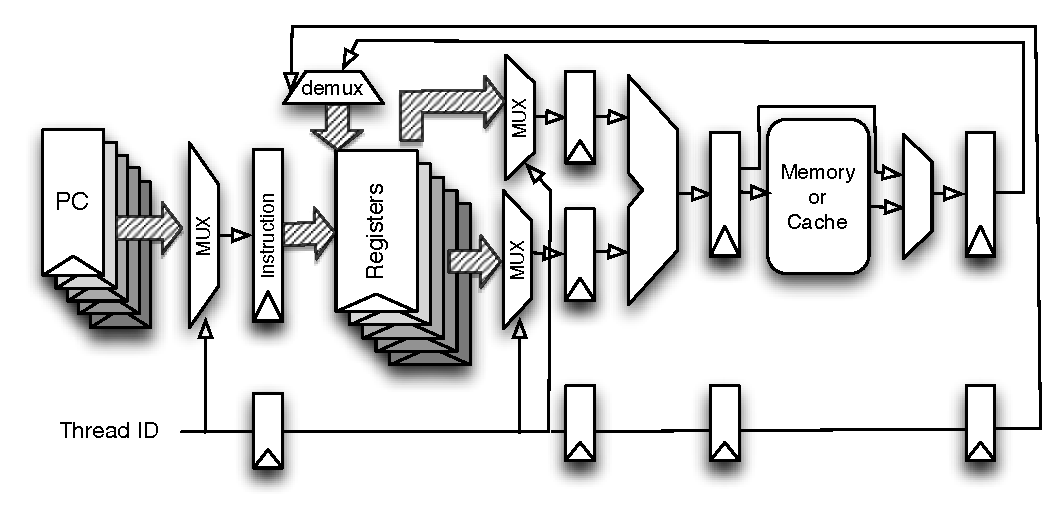
\includegraphics[scale=.8]{figs/multithreaded_pipeline_block}
\end{center}
\vspace{-30pt}
\caption{Simple Multithreaded Pipeline}
\label{fig:multi-thread pipeline simplified}
\end{figure}
Figure~\ref{fig:multi-thread pipeline simplified} shows a architectural level view of a simple multithreaded pipeline.
It contains 5 hardware threads, so it has 5 copies of the Program Counter (PC) and Register files.
Once a hardware thread is executing in the pipeline, its corresponding thread state can be selected by signaling the correct selection bits to the multiplexers.
The rest of the pipeline remains similar to a traditional 5 stage pipeline as introduced in Hennessy and Pattern\todo{citation}.   
The extra copies of the thread state and the multiplexers used to select them thus contribute to most of the hardware additions needed to implement hardware multithreading.

%The selection of threads for execution is one of the most important factors to fully utilize thread-level parallelism.
%If a thread is stalled waiting for memory access but gets selected to execute in the pipeline, then that instruction slot is wasted and the processor isn't fully utilized.
Ungerer et al.~\cite{Ungerer:2003:survey_multithreading} surveyed different multithreaded architectures and categorized them based upon the \todo{thread selection?} policy and the execution width of the pipeline.
The thread selection policy is the context switching scheme used to determine which threads are executing, and how often a context switch occurs.  
Coarse-grain policies manage hardware threads similar to the way operation systems manage software threads.
A hardware thread gain access to the pipeline and continues to execute until a context switch is triggered.
Context switches occur less frequently via this policy, so less hardware threads are required to fully utilize the processor.
Different coarse-grain policies trigger context switches with different events. 
Some trigger on dynamic events, such as cache miss or interrupts, and some trigger on static events, such as specialized instructions.
Fine-grain policies switch context much more frequently -- usually every processor cycle.
Both coarse-grain and fine-grain policies can also have different hardware thread scheduling algorithms that are implemented in a hardware thread scheduling controller to determine which hardware thread is switched into execution.  
The width of the pipeline refers to the number of instructions that can be fetched into execution in one cycle. 
For example, superscalar architectures have redundant functional units, such as multipliers and ALUs, and can dispatch multiple instructions into execution in a single cycle. 
Multithreaded architectures with pipeline widths of more than one, such as Sumultanous Multithreaded (SMT) architectures, can fetch and execute instructions from several hardware threads in the same cycle.

Multithreaded architectures typically bring additional challenges to execution time analysis of software running on them.
Any timing analysis for code running on a particular hardware thread needs to take into account not only the code itself, but also the thread selection policy of the architecture and sometimes even the execution context of code running on other hardware threads.
For example, if dynamic coarse-grain multithreading is used, then a context switch could occur at any point when a hardware thread is executing in the pipeline.
This not only has an effect on the control flow of execution, but also the state of any hardware that is shared, such as caches or branch predictors.    
Thus, it becomes nearly impossible to estimate execution time without knowing the exact execution state of other hardware threads and the state of the thread scheduling controller.
However, it is possible to for multithreaded architectures to fully utilize thread-level parallelism while still maintaining timing predictability.
Thread-interleaved pipelines use a fine-grain thread switching policy with round robin thread scheduling to achieve high instruction throughput while still allowing precise timing analysis for code running on its hardware threads. 
Below, its architecture and trade-offs are described and discussed in detail along with examples and explanation of how timing predictability is maintained.
Through the remainder of this chapter, we will use the term ``thread'' to refer to explicit hardware threads that have physically separate register files, program counters, and other thread states.
This is not to be confused the common notion of ``threads'', which is assumed to be software threads that is managed by operating systems with thread states stored in memory.

\subsection{Thread-Interleaved Pipelines}
\label{subsection:pret_thread_pipeline}
\begin{figure}
  \vspace{-20pt}
  \begin{center}
    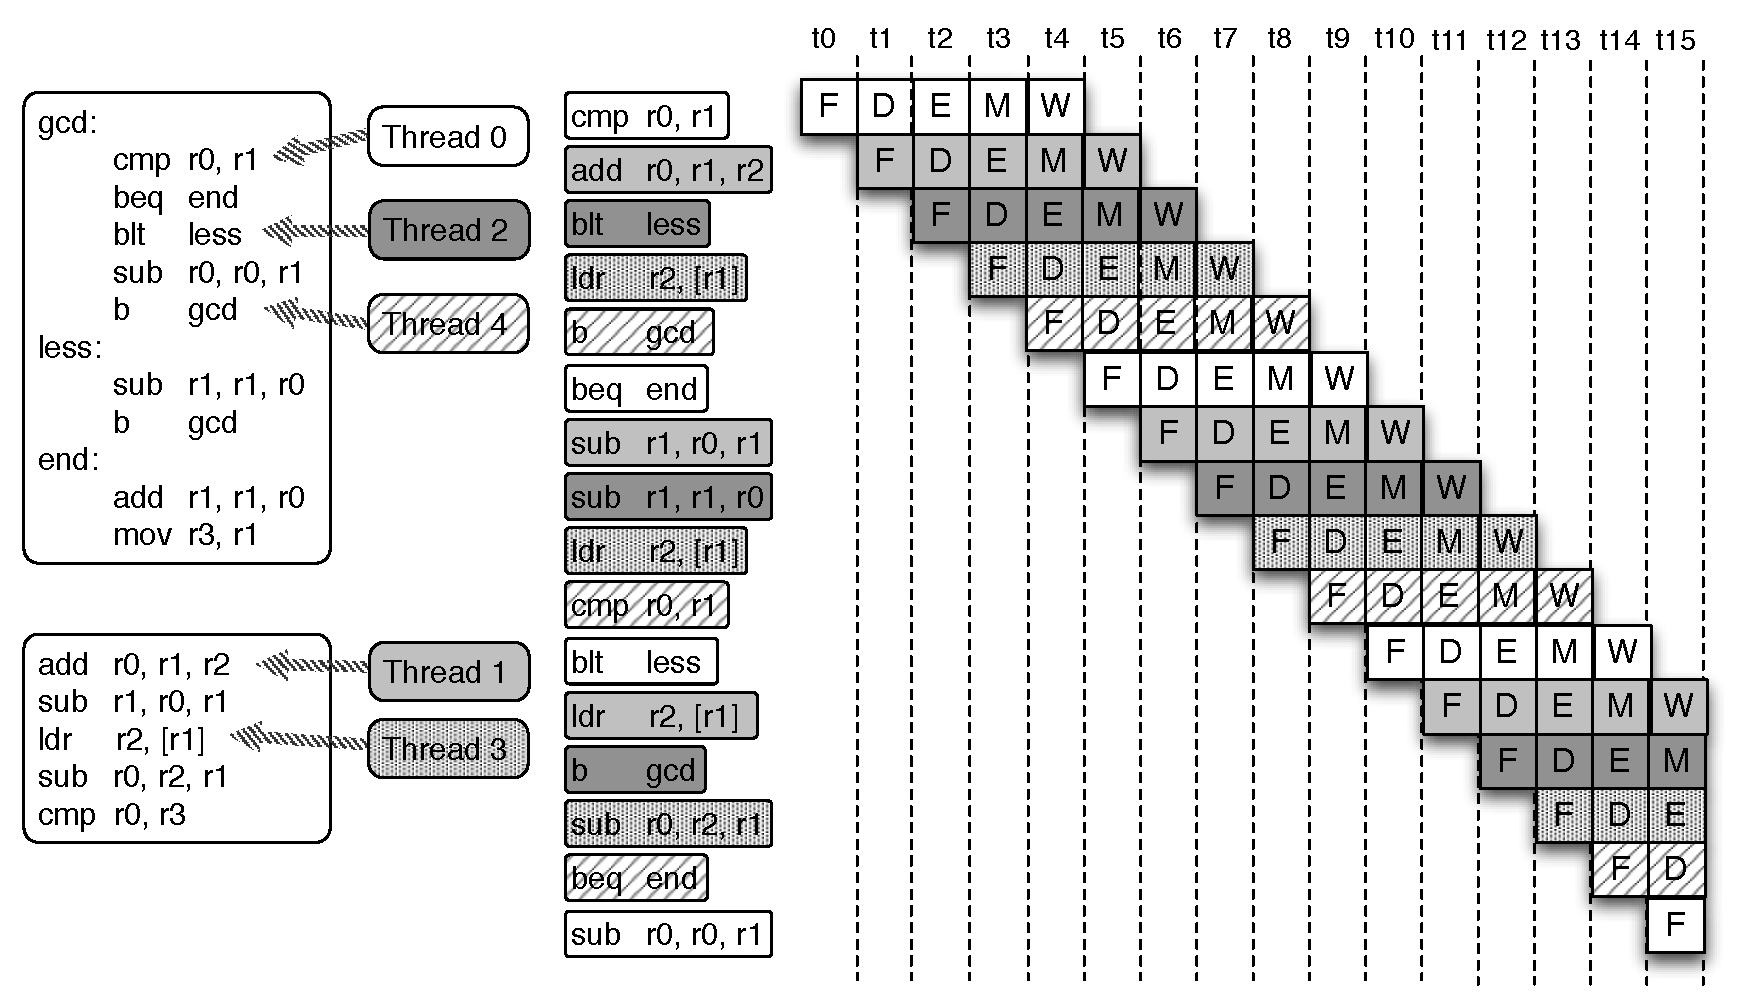
\includegraphics[scale=.55]{figs/thread-interleaved-execution}
  \end{center}
  \vspace{-20pt}
  \caption{Sample execution sequence of a thread-interleaved pipeline with 5 threads and 5 pipeline stages}
  \label{fig:execution_thread_interleaved_pipeline}
\end{figure}
The thread-interleaved pipeline was introduced to improve the response time of handling multiple I/O devices \todo{citation}.
I/O operations often stall from the communication with the I/O devices.
Thus, interacting with multiple I/O devices leads to wasted processor cycles that are idle waiting for the I/O device to respond.
By employing multiple hardware thread contexts, a hardware thread stalled from the I/O operations does not stall the whole pipeline, as other hardware threads can be fetched and executed.
% In a thread-interleaved pipeline, a thread context switch occurs every processor cycle, and the threads are cycled through in a round robin fashion. 
% This ensures each thread gets equal access to the process resource, so threads that aren't stalled are guaranteed to make progress.
Thread-interleaved pipelines use fine-grain multithreading; every cycle a context switch occurs and a different hardware thread is fetched into execution. 
The threads are scheduled in a deterministic round robin fashion. 
This also reduces the context switch overhead down to nearly zero, as no time is needed to determine which thread to fetch next, and barely any hardware is required to implement round robin thread scheduling; a simple $log(n)$ bit up counter (for $n$ threads) would suffice.         
Figure~\ref{fig:execution_thread_interleaved_pipeline} shows an example execution sequence from a 5 stage thread-interleaved pipeline with 5 threads.
The thread-interleaved pipelines shown and presented in this thesis are all of single width.
The same code segments from figure~\ref{fig:sample_gcd_code} and figure~\ref{fig:sample_data_dependent_code} are being executed in this pipeline. 
Threads 0, 2 and 4 execute GCD (figure~\ref{fig:sample_gcd_code}) and threads 1 and 3 execute the data dependent code segment (figure~\ref{fig:sample_data_dependent_code}).
Each hardware thread executes as an independent context.
Their progress is shown in figure~\ref{fig:execution_thread_interleaved_pipeline} with thick arrows pointing to the execution location of each thread at t0.    
We can observe from the figure that each time step an instruction from a different hardware thread is fetched into execution and the hardware threads are fetched in a round robin order.
At time step 4, the processor is completely filled, and each pipeline stage is occupied by a different hardware thread.
This remains the same for time step 5, 6, 7 and so on. 
The fine-grained thread interleaving and the round robin scheduling combine to form this unique property of thread-interleaved pipelines, which provides the basis for a timing predictable architecture design.

For thread-interleaved pipelines, if there are, at a minimum, the same number of threads as there are pipeline stages, then the data-dependencies that were caused from pipelining no longer exist. 
We will use the term ``full'' thread-interleaved pipelines if there exists at least the same number of threads in the pipeline as pipeline stages.  
%With $n$ threads occupying a $n$ stage pipeline, we remove the data-dependencies caused by the pipeline.
Dependencies arise when an instruction needs data from another instruction that is currently executing in the pipeline and has not yet completed its execution.
As illustrated in figure~\ref{fig:execution_thread_interleaved_pipeline}, instructions in a full thread-interleaved pipeline can never be dependent upon any other instruction that's currently in executing in the pipeline, because each stage of the pipeline is occupied by an instruction from a different thread.
In other words, an instruction will always commit before the next instruction from the same thread is fetched, thus no data-dependency within instructions can occur. 


For instructions that take multiple cycles, a replay mechanism is used so the round robin thread scheduling is preserved and no interference is introduced between the threads.
When a multi-cycle instruction is fetched into the pipeline from a thread, it executes as any instruction.
As the instruction goes through the pipeline, no results are committed, but instead its state is saved in a hardware thread control block and does not increment the program counter for this thread. 
When an instruction fetch from this thread occurs, the same instruction is dispatched into the pipeline to continue its execution. 
If it still has not completed its execution, then the program counter for this thread is again not incremented and the same instruction is dispatched, until it is completed. 
%FIXME: Place in replay mechanism figure
For instructions that take multiple cycles due to limitations of the pipeline design, this mechanism makes sense.
Instructions that do 64-bit operations on a 32-bit pipeline datapath for example falls into this category. 
In order to abide to the round-robin thread scheduling, the thread simply saves the instruction state and continues execution when it gains access to the pipeline. 
However, for other multi-cycle instructions, such as memory operations, this mechanism might seem counter intuitive. 
These instructions require multiple cycles because data is required from other hardware components that have longer access latencies.
Memory operations or floating point operations are categorized into such instructions because they are waiting for data from main memory access or computation results from floating point units.
Often times multithreaded architectures mark these threads inactive and the thread is not rescheduled until the data is ready.
This is done to maximize the throughput of the pipeline, since threads waiting for data from other hardware components cannot make any progress until the data is returned. 
However, this leads to unpredictable timing behaviors in the threads.
When threads are scheduled and unscheduled dynamically, the other threads in the pipeline would dynamically execute more or less frequently depending on which threads are active and inactive.
This greatly complicates any timing analysis on the software running on each thread as the execution frequency of the threads would depend on the execution of other threads.
Thus, our thread-interleaved pipeline does not mark threads inactive, but simply replays the instruction from the thread.
The effects of latency hiding is still present, as other threads continue to progress while one thread is replaying its multi-cycle instruction.  

%fixme: Add floating point unit description
Care must also be taken when adding datapaths that take multiple cycles, or else the interference introduced could easily disrupt the timing analysis of threads.
If the added datapath isn't able to support pipelined or simultaneous operations, then it will introduce contention amongst the threads.
For example, in figure~\ref{fig:none_pipelined_floatingpoint} we show the effects of adding a non-pipelined floating point divider that takes 20 cycles to execute.    
\begin{figure}
\begin{center}

\includegraphics[scale=.4]{figs/placeholder}
\end{center}
\caption{None Pipelined Floating Unit}
\label{fig:none_pipelined_floatingpoint}
\end{figure}
As one thread executes a floating-point division instruction, any other thread that also executes a floating-point division must now wait until the first instruction finishes. 
If other threads also executes the same instruction, then queuing mechanisms must be introduced, for threads that are contending for the floating-point divider. 
This would greatly complicate the timing analysis, as the execution time of floating-point division instructions now depend on the execution context of other threads.
Pipelining the floating-point divider would increase the throughput at the cost of area and latency. 
However, by pipeling the floating-point divider unit, each thread that executes a floating-point division can now access it without contention. 
The replay mechanism also hides the long latency of the instruction, and benefits from the improved latency. 
Because there is no contention, the timing analysis of floating-point operations are now trivial and predictable.     

In summary, blah blah blah\ldots
\subsection{Memory System}
\label{subsection:memory_system}


\section{Implementation}
\subsection{PTARM Simulator}
\label{subsection:ptarm_sim}

\subsection{PTARM VHDL Softcore}
\label{subsection:ptarm_vhdl_softcore}

\subsection{Worst Case Execution Time Analysis}
\label{sec:wcet}